\chapter{This Is The First Chapter}
\section{And The First Section}
This is a Cobb-Douglas functions, very useful in Economics:
\begin{equation}
	y = x_{1}^{\alpha}x_{2}^{\beta}
\end{equation}

Here is an example of a piece of R code inside the listing environment.
\begin{lstlisting}
> pro <- rnorm(100)
> summary(pro)
    Min.  1st Qu.   Median     Mean  3rd Qu.     Max. 
-2.71000 -0.75030 -0.01813 -0.03029  0.62060  2.49600 
> plot(pro)
\end{lstlisting}
This code generates a sample of 100 pseudo-random numbers from a Normal distribution, with the summary functions we have some descriptive statistics and by plot functions we obtain a graphical representation of that data.

Here is the plot:
\begin{figure}[th]
	\centering
	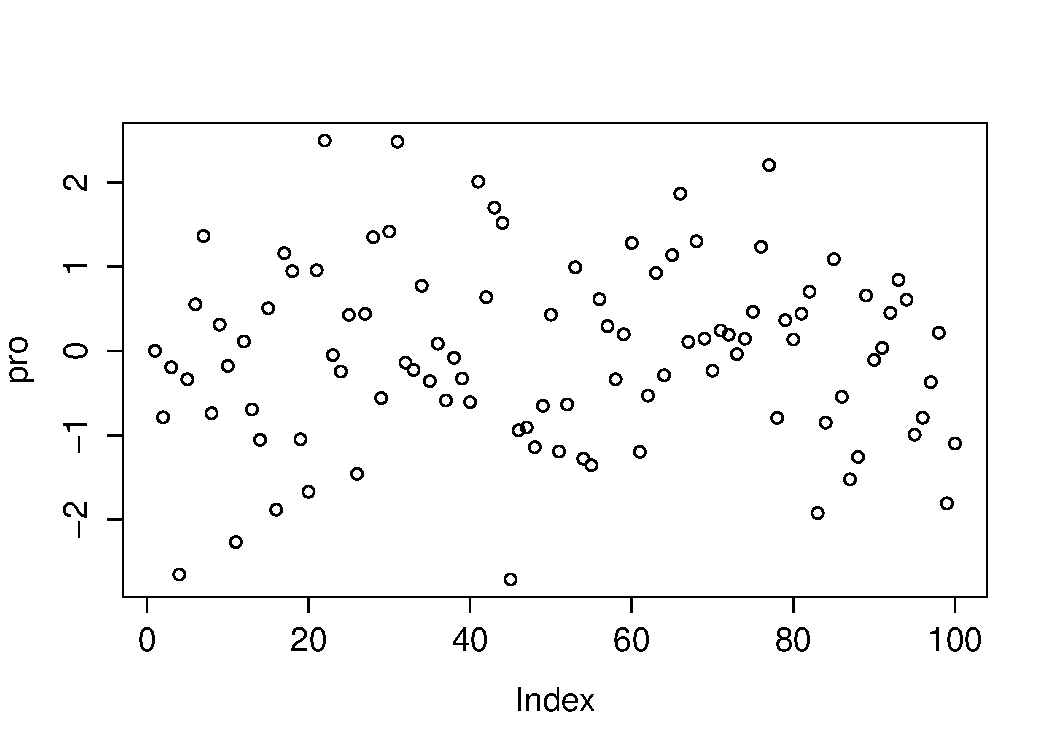
\includegraphics[width=\textwidth]{pictures/Rplot.pdf} 
	\caption[Sample from a Normal]{Here is the sample of 100 pseudo-numbers 	from a Normal distribution.}
\end{figure}
\section{And The Second Section}
\lipsum